\documentclass[../../script.tex] {subfiles}
%! TEX root = ../../script.tex

\begin{document}
\section{Open and Closed Sets}

\begin{defi}[Inner points and Boundary points]
    Let $\metric$ be a metric space, $A \subset X$ and $x \in X$. 
    \begin{enumerate}[(i)]
        \item $x$ is said to be an inner point of $A$, if \[ \exists \epsilon > 0: ~~ \oball(x) \subset A \]
        \item $x$ is said to be a boundary point of $A$ if 
        \[
            \forall \epsilon > 0: ~~\underbrace{\oball(x) \cap A \ne \emptyset}_{\substack{\oball(x) \text{ contains} \\ \text{points from } A}}
            \wedge \underbrace{\oball(x) 
            \cap (X \setminus A) \ne \emptyset}_{\substack{\oball(x) \text{ contains points}\\ \text{from outside of } A}}
        \]
        \item The set 
        \[
            \set[x \text{ is inner point of } A]{x \in X}
        \]
        is called the interior of $A$, and is denoted as $\interior{A}$.
        \item The set 
        \[
            \set[x \text{ is boundary point of} A]{x \in X}
        \]
        is called the boundary of $A$, and is denoted as $\partial A$.
        \item $A \cup \boundary{A}$ is said to be the closure of $A$, and is denoted as $\closure{A}$.
    \end{enumerate}
        
        \begin{center}
            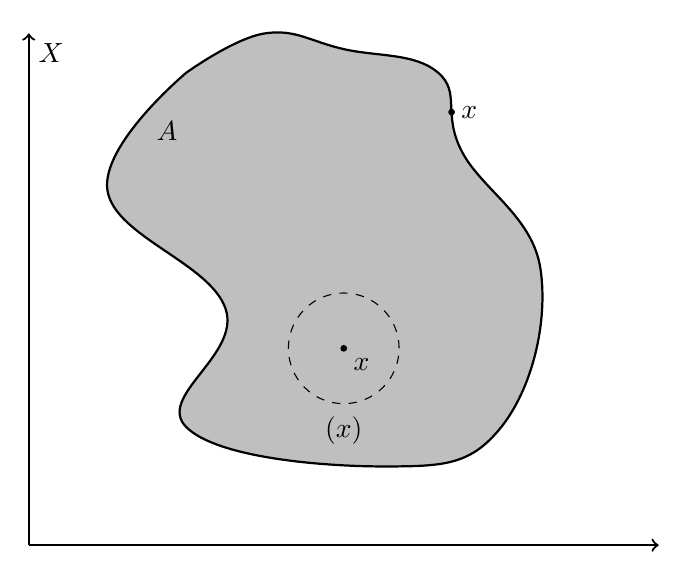
\begin{tikzpicture}
                \draw [->, thick] (-6, -3.5) -- (-6, 3);
                \draw [->, thick] (-6, -3.5) -- (2, -3.5);
                \draw [thick, fill=lightgray]  plot[smooth, tension=.7] coordinates {(-4,2.5) (-3,3) (-2,2.8) (-0.8,2.5) (-0.5,1.5) (0.5,0) (0,-2)(-1.5,-2.5) (-4,-2) (-3.5,-0.5) (-5,1) (-4,2.5)};
            
                \node[below right] at (-6, 3) (X) {$X$};
                \node[below right] at (-4.5, 2) (A) {$A$};
    
                \draw[fill] (-2, -1) circle [radius=1pt];
                \node[below right] at (-2, -1) (C) {$x$};
                \draw[dashed] (-2, -1) circle [radius=20pt];
                \node[below] at (-2, -1.75) (C) {$\oball(x)$};
    
                \draw[fill] (-0.63, 2) circle [radius=1pt];
                \node[right] at (-0.63, 2) (C) {$x$};
            \end{tikzpicture}
        \end{center}
\end{defi}

\begin{eg}
    Consider $X = \realn^2$. Then 
    \begin{align*}
        A &= \set[0 \le y < 1]{(x, y) \in \realn} \\
        \mathring{A} &= \set[0 \le y < 1]{(x, y) \in \realn^2} \\
        \boundary{A} &= \set[y = 1 \vee y = 0]{(x, y) \in \realn^2} \\
        \closure{A} &= \set[0 \le y \le 1]{(x, y) \in \realn^2}
    \end{align*}
\end{eg}

\begin{rem}
    \begin{enumerate}[(i)]
        \item $\interior{A} \subset A$
        \item Boundary points of $A$ can be elements of $A$ or not.
        \item $A \subset \interior{A} \cup \boundary{A}$, $~~\interior{A} \cap \boundary{A} = \varnothing$
        \item $\boundary{A} = \boundary{X \setminus A}$
    \end{enumerate}
\end{rem}

\begin{thm}
    Let $\metric$ be a metric space, $A \subset X$ and $x$ an interior point or boundary point of $A$. Then 
    \[
        \exists \anyseqdef{A}: ~~x_n \conv{} x
    \]
\end{thm}
\begin{proof}
    If $x \in A$ then this is trivial, so let $x \notin A$. Then 
    \begin{equation}
        \forall n \in \natn ~\exists x_n \in \left(\oball[\frac{1}{n}](x) \cap A \ne \varnothing\right)
    \end{equation}
    We need to show that $\seq{x}$ converges to $x$.
    \begin{equation}
        \forall \epsilon > 0 ~\epsilon N \in \natn: ~~\frac{1}{N} < \epsilon
    \end{equation}
    For $n \ge N$ we have 
    \begin{equation}
        \frac{1}{n} \le \frac{1}{N} < \epsilon
    \end{equation}
    and thus 
    \begin{equation}
        d(x_n, x) < \frac{1}{n} < \epsilon
    \end{equation}
\end{proof}

\begin{defi}[Open and Closed sets]
    Let $\metric$ be a metric space. $A \subset X$ is said to be 
    \begin{enumerate}[(i)]
        \item open, if every point in $A$ is an interior point
        \item closed, if $A$ contains all its boundary point 
        \item neighbourhood of $x \in A$, if $x$ is an interiot point of $A$
    \end{enumerate}
\end{defi}

\begin{thm}
    Let $\metric$ be a metric space and $A \subset X$.
    \[
        A \text{ open} \iff X \setminus A \text{ closed}
    \]
\end{thm}
\begin{proof}
    \begin{subequations}
    \begin{align}
        A \text{ open} &\iff \forall x \in A: ~~x \in \interior{A} \\
        &\iff \forall x \in A: ~~x \in \boundary{A} \\
        &\iff X \setminus A \text{ contains all boundary point of } A \\
        &\iff X \setminus A \text{ contains all boundary points of } X \setminus A \\
        &\iff X \setminus A \text{ closed}
    \end{align}
    \end{subequations}
\end{proof}

\begin{rem}
    That doesn't mean $A$ has to be either open and closed.
\end{rem}

\begin{eg}
    Let $\metric$ be a metric space, $x \in X$ and $r > 0$. Then 
    \begin{align*}
        \Oball(x) &= \set[d(x, y) < r]{y \in X} \text{ is open} \\
        \Cball(x) &= \set[d(x, y) < r]{y \in X} \text{ is closed}
    \end{align*}
\end{eg}

\begin{rem}
    Consider the special case $a, b \in \realn$ with $a < b$
    \begin{align*}
        (a, b) &= \oball[\frac{b - a}{2}]\left(\frac{a + b}{2}\right) \text{ open} \\
        [a, b] &= \cball[\frac{b - a}{2}]\left(\frac{a + b}{2}\right) \text{ closed}
    \end{align*}
\end{rem}

\begin{thm}
    Let $\metric$ be a metric space and $A \subset X$. 
    \[
        A \text{ closed} \iff \forall \anyseqdef{A} \text{ convergent}: ~~\limn{x_n} \in A
    \]
\end{thm}
\begin{proof}
    Assume $A$ is closed. Let $\anyseqdef{A}$ be convergent to $x$. then
    \begin{equation}
        \forall \epsilon > 0 ~\exists N \in \natn: ~~x_n \in \oball(x) ~~\forall n \ge N
    \end{equation}
    This means that every $\epsilon$-ball around $x$ contains at least one point from $A$.
    I.e. $x$ is always a point (or a boundary point) of $A$. From $A$ closed follows $x \in A$.

    Now assume $x \in \boundary{A}$. Then 
    \begin{equation}
        \exists \anyseqdef{A}: ~~\seq{x} \conv{} x
    \end{equation}
    According to the prerequisites, $x \in A$.
\end{proof}

\begin{thm}
    Let $\metric$ be a metric space, and $\tau$ the set of all open subsets. Then 
    \begin{enumerate}[(i)]
        \item $\varnothing \in \tau$, $~~X \in \tau$
        \item The union of any number of sets from $\tau$ is an open set
        \[
            \bigcup_{t \in \tau} t \in \tau
        \]
        \item The intersection of finitely many sets from $\tau$ is an open set 
        \[
            \bigcap_{t \in \tau} t \in \tau
        \]
    \end{enumerate}
\end{thm}
\begin{proof}
    \reader
\end{proof}

\begin{rem}
    \begin{enumerate}[(i)]
        \item $\tau$ is said to be the topology induced by $d$
        \item \begin{itemize}
            \item $\varnothing$, $X$ are also closed 
            \item The intersection of any number of closed sets is closed 
            \item The union of finitely many closed sets is closed 
        \end{itemize}
        \item Infinitely many intersections of open sets are not open in general.
    \end{enumerate}
\end{rem}

\begin{thm}
    Let $\metric$ be a metric space and $A \subset X$. Then 
    \[
        \interior{A} \text{ open} \implies \boundary{A}, \closure{A} \text{ closed}
    \]
\end{thm}
\begin{proof}
    Let $\interior{A}$ be open and $x \in \interior{A} \subset A$. This means 
    \begin{equation}
        \exists \epsilon > 0: ~~\oball(x) \subset A
    \end{equation}
    We have to show that $\oball(x) \subset \interior{A}$. Let $y \in \oball(x)$. 
    Since $\oball(x)$ is open
    \begin{equation}
        \exists \delta > 0: ~~\oball[\delta](y) \subset \oball(x) \subset A
    \end{equation}
    This means that $y \in \oball(x)$ is interior point $A$. I.e. $\subset(x) \subset \interior{A}$, and thus $x$ is interior point of $\interior{A}$.

    Let $B = X \setminus A$. Then $\boundary{A} = \boundary{B}$
    \begin{equation}
        X = A \cup B = \interior{A} \cup \boundary{A} \cup \interior{B} \cup \boundary{B} = \interior{A} \cup \boundary{A} \cup \interior{B}
    \end{equation}
    Then 
    \begin{subequations}
    \begin{align}
        A \text{ and } B \text{ are disjoint } &\implies \interior{A}, \interior{B} \text{ disjoint} \\
        &\implies \boundary{A} \text{ disjoint to } \interior{A}, \interior{B}
    \end{align}
    \end{subequations}
    This results in 
    \begin{equation}
        \boundary{A} = X \setminus (\underbrace{\interior{A} \cup \interior{B}}_{\text{open}}) \implies \boundary{A} \text{ closed}
    \end{equation}
    and 
    \begin{equation}
        \closure{A} = A \cup \boundary{A} = \interior{A} \cup \boundary{A} = X \setminus \interior{B} \text{ closed}
    \end{equation}
\end{proof}

\begin{thm}
    Let $\metric$ be a metric space and $A \subset X$
    \begin{align*}
        \bigcup_{\substack{O \text{ open} \\ O \subset A}} O = \interior{A} && \text{and} && \bigcap_{\substack{C \text{ closed} \\ A \subset C}} C = \closure{A}
    \end{align*}
\end{thm}
\begin{proof}
    Let $\interior{A}$ is open and $\interior{A} \subset A$
    \begin{equation}
        \implies \bigcup_{O \subset A \text{ open}} \supset \interior{A}
    \end{equation}
    Now let $O \subset A$ be open and $x \in O$, i.e.
    \begin{equation}
        \exists \epsilon > 0: ~~\oball(x) \subset O \subset A \implies x \in \interior{A}
    \end{equation}
    This implies that $O \subset \interior{A}$. Since this holds for all open $O \subset A$, this statement is proven.
    The other statement follows from the complement.
\end{proof}

\begin{thm}
    Let $\metric$ be a complete space and $A \subset X$ be closed. Then $(A, d_A)$ is complete.
\end{thm}
\begin{proof}
    \reader
\end{proof}

\begin{rem}
    Topological terms (open, closed, continuous, compact) don't just depend on $A$, but also on $X$.
\end{rem}

\begin{defi}
    Let $\metric$ be a metric space and $x \in X$.
    \begin{enumerate}[(i)]
        \item $x$ is said to be an isolated point if $\exists \epsilon > 0$ such that $\oball(x) = \set{x}$.
        \item $x$ is said to be a limit point if it's not an isolated point.
    \end{enumerate}
\end{defi}

\begin{defi}[Punctured neighbourhood, Punctured ball]
    $\dot{U} \subset X$ is said to be a punctured neighbourhood, if there is a neighbourhood $U$ of $x$ with $\dot{U} = U \setminus \set{x}$

    A punctured ball is $\dot{\oball}(x) = \oball \setminus \set{x}$.
\end{defi}

\begin{defi}[Limit of mappings]
    Let $(X, d_X), (Y, d_Y)$ and $x$ a limit point of $X$. Let $\dot{U}$ be a punctured neighbourhood of $x$ and $f: \dot{U} \rightarrow Y$.
    Then $f$ converges to $y \in Y$ in $x$ ($y$ is said to be the limit of $f$ in $x$), if 
    \[
        \forall \epsilon > 0 ~\exists \delta > 0: ~~f(\tilde{x}) \in \oball(y) ~~[d(f(\tilde{x}), y) < \epsilon]
    \]
    if $\tilde{x} \in \dot{\oball}(x)$ [$d(\tilde{x}, x) < \delta$]
\end{defi}

\begin{eg}
    Let $f, g: \realn^2 \setminus \set{0} \rightarrow \realn$.
    \begin{align*}
        f(x) := \norm{x}^2 && g(x) := \frac{1}{\norm{x}}
    \end{align*}
    Then $\limes{x}{0} f(x) = 0$, because for $\epsilon > 0$ and $\delta = \sqrt{\epsilon}$ we have 
    \[
        d(\tilde{x}, 0) = \norm{\tilde{x} - 0} = \tilde{x} < \delta \implies d(f(\tilde{x}), 0) = \abs{\norm{\tilde{x}}^2 - 0} = \norm{\tilde{x}}^2 < \epsilon = \delta^2
    \]
\end{eg}

\begin{thm}
    \[ 
        f \text{ converges to } y \in Y \text{ in } x \iff \forall \anyseqdef{X}: ~~f(x_n) \conv{x_n \rightarrow x} y
    \]
\end{thm}
\begin{proof}
    Let $\anyseqdef{X}$ with $x_n \conv{} x$. Let $\epsilon > 0$, then 
    \begin{equation}
        \exists \delta > 0: ~~f(\tilde{x}) \in \oball(y) \text{ if } \tilde{x} \in \oball[\delta](x)
    \end{equation}
    Furthermore
    \begin{equation}
        \exists N \in \natn: ~~x_n \in \oball[\delta](x) ~~\forall n \ge N
    \end{equation}
    Then 
    \begin{equation}
        f(x_n) \in \oball(y) ~~\forall n \ge N
    \end{equation}
    To prove the other direction, assume $f$ doesn't converge to $y$ in $y$. This means 
    \begin{equation}
        \exists \epsilon > 0: ~~\exists \tilde{x} \in \oball[\delta](x) \text{ but } f(\tilde{x}) \notin \oball(y) ~~\forall \delta > 0
    \end{equation}
    Therefore 
    \begin{equation}
        \forall n \in \natn: ~~\exists x_n \in \oball[\frac{1}{n}](x)
    \end{equation}
    We know that $x_n \conv{} x$ since $d(x_n, x) < \frac{1}{n}$, but $f(x_n)$ doesn't converge to $y$ since $d(f(x_n), y) \ge \epsilon$.
\end{proof}

\begin{cor}
    Let $\metric$ be a metric space, $x \in X$ a limit point and $\dot{U}$ a punctured neighbourhood of $x$. Let $f, g: \dot{U} \rightarrow \field$ with 
    \begin{align*}
        \limes{\tilde{x}}{x} f(\tilde{x}) = y_1 && \limes{\tilde{x}}{x} g(\tilde{x}) = y_2
    \end{align*}
    Then 
    \begin{align*}
        \limes{\tilde{x}}{x} (f + g)(\tilde{x}) = y_1 + y_2 && \limes{\tilde{x}}{x} (f \cdot g)(\tilde{x}) = y_1 \cdot y_2 \\
        \limes{\tilde{x}}{x} \left(\frac{f}{g}\right)(\tilde{x}) = \frac{y_1}{y_2}
    \end{align*}
\end{cor}
\begin{hproof}
    Draw parallels back to number sequences
\end{hproof}
\end{document}